\documentclass[twocolumn,11pt]{sotsuken_abst}
\usepackage{amsmath}
\usepackage{flow}
\usepackage[dvipdfmx]{color}
\usepackage[dvipdfmx]{graphicx}




% タイトル
\title{音声認識を用いて接客をするロボットの開発}

\author{澤田茂人(指導教員 伊藤恒平)}

%\urlstyle{rm}

\setcounter{page}{1}
\lhead{}
\chead{}
\rhead{{\sf 16・201}\\{\bf 機械工学科}}
\lfoot{}
\cfoot{{\sf-\ M-\thepage \ -}}
%\rfoot{}
\renewcommand{\headrulewidth}{3pt}
%\renewcommand{\footrulewidth}{1pt}



\begin{document}
%\layout
\maketitle
\thispagestyle{fancy}
\pagestyle{fancy}

\setlength{\baselineskip}{5.6truemm}
\kanjiskip=.07zw plus 3pt minus 3pt
\xkanjiskip=.07zw plus 3pt minus 3pt
\begin{document}


\maketitle
%%%%%%%%%%%%%%%%%%%%%%%%%%%%%%%%%%%%%%%%%%%%%%%%%%%%%%%%%%%%%%%%%%%%%%%%%%%%%%%%
\section{はじめに}
\subsection{研究の背景}
近年,飲食店において接客をロボット化する事により経費を削減したいとの要望がある.そこで音声でのやりとりをするためのシステムを究明する必要があると考え,本研究を開始した.飲食店で注文を取るロボットに使用した音声を認識させるシステムについて今から述べていく.
\subsection{研究の目的}
飲食店にてPCを実装したロボットに音声認識をするためJulius,Open-JTalk,認識すべき単語,マイクを準備し飲食店で禁煙か喫煙かの判断や「あちらの席へどうぞ」「こちらの席へどうぞ」のようなレベルの案内をすることを目的とする.図\ref{fig:yousu}に音声認識をしようとしたときのイメージ図を示す.

\begin{figure}[htbp]
\begin{center}
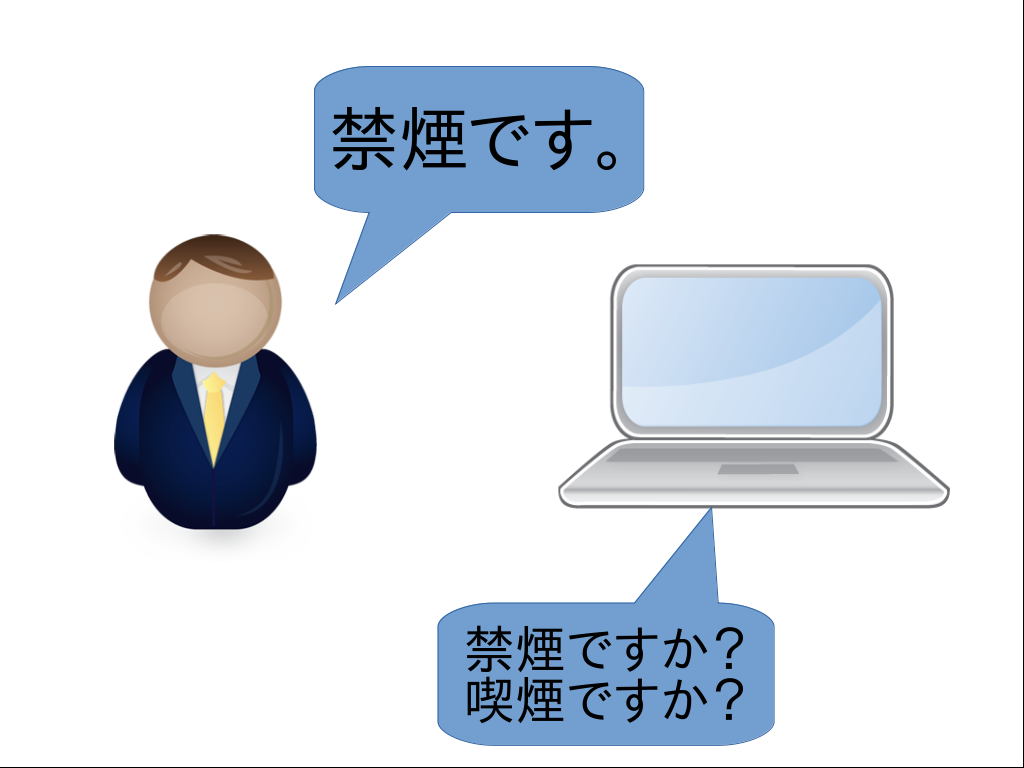
\includegraphics[width=35mm]{img/Image.png}
\caption{様子}
\label{fig:yousu}
\end{center}
\end{figure}

\section{飲食店での接客について}
\subsection{接客の仕事内容}
お客さまから注文を取り,出来上がった料理や飲み物を運び,空いた皿の片付け,レジ業務を行うのが主な仕事である.その接客の仕事内容を図\label{fig:customer-service}のフローチャートに示す.

\documentstyle
\begin{document}
\scriptsize
\setiftext{yes}{no}
\STRUCT{開始}{}{%
    \ACTION{\centering{お出迎えする.}}%
    \ACTION{人数の確認.}%
        \CASE{禁煙喫煙の確認.}{%
        \WHEN{禁煙の場合}{%
            \ACTION{\centering{あちらの席へどうぞ.}}%
        }%
        \WHEN{喫煙の場合}{%
            \ACTION{\centering{こちらの席へどうぞ.}}%
        }%
        \WHEN{5人以上の客でなおかつ禁煙の場合}{%
            \ACTION{\centering{「ただいま席をお作りしますので少しお待ちください.」}}%
        }%
    }%
    \ENDCASE%
    \ACTION{\centering{オーダーを取る.}}%
    \ACTION{\centering{料理を出す.}}%
    \ACTION{\centering{レジで会計を行う.}}%
}%
\caption{接客方法の流れ}%
\label{fig:customer-service}%
\normalsize


\subsection{研究として検討する接客の業務内容}
図に示した一連の接客内容を研究として再現するのは難しい.したがって,今年度は再現する箇所を絞り,出迎え作業を検討することとした.出迎え作業とはお客様を待つために入口付近で待機していなければならない.しかし,その業務をロボット化した場合入口付近で待機している時間の経費を削減できると考えた.そこで,店の入口付近で客がタバコを吸うかどうかの判断や「あちらの席へどうぞ」「こちらの席へどうぞ」の案内をすることが研究として検討する仕事となる.


\section{検討用のシステムについて}
今年度のシステムは図\ref{fig:robot}に示すシステムを使用して音声認識を行う.


\begin{figure}[htbp]
\begin{center}
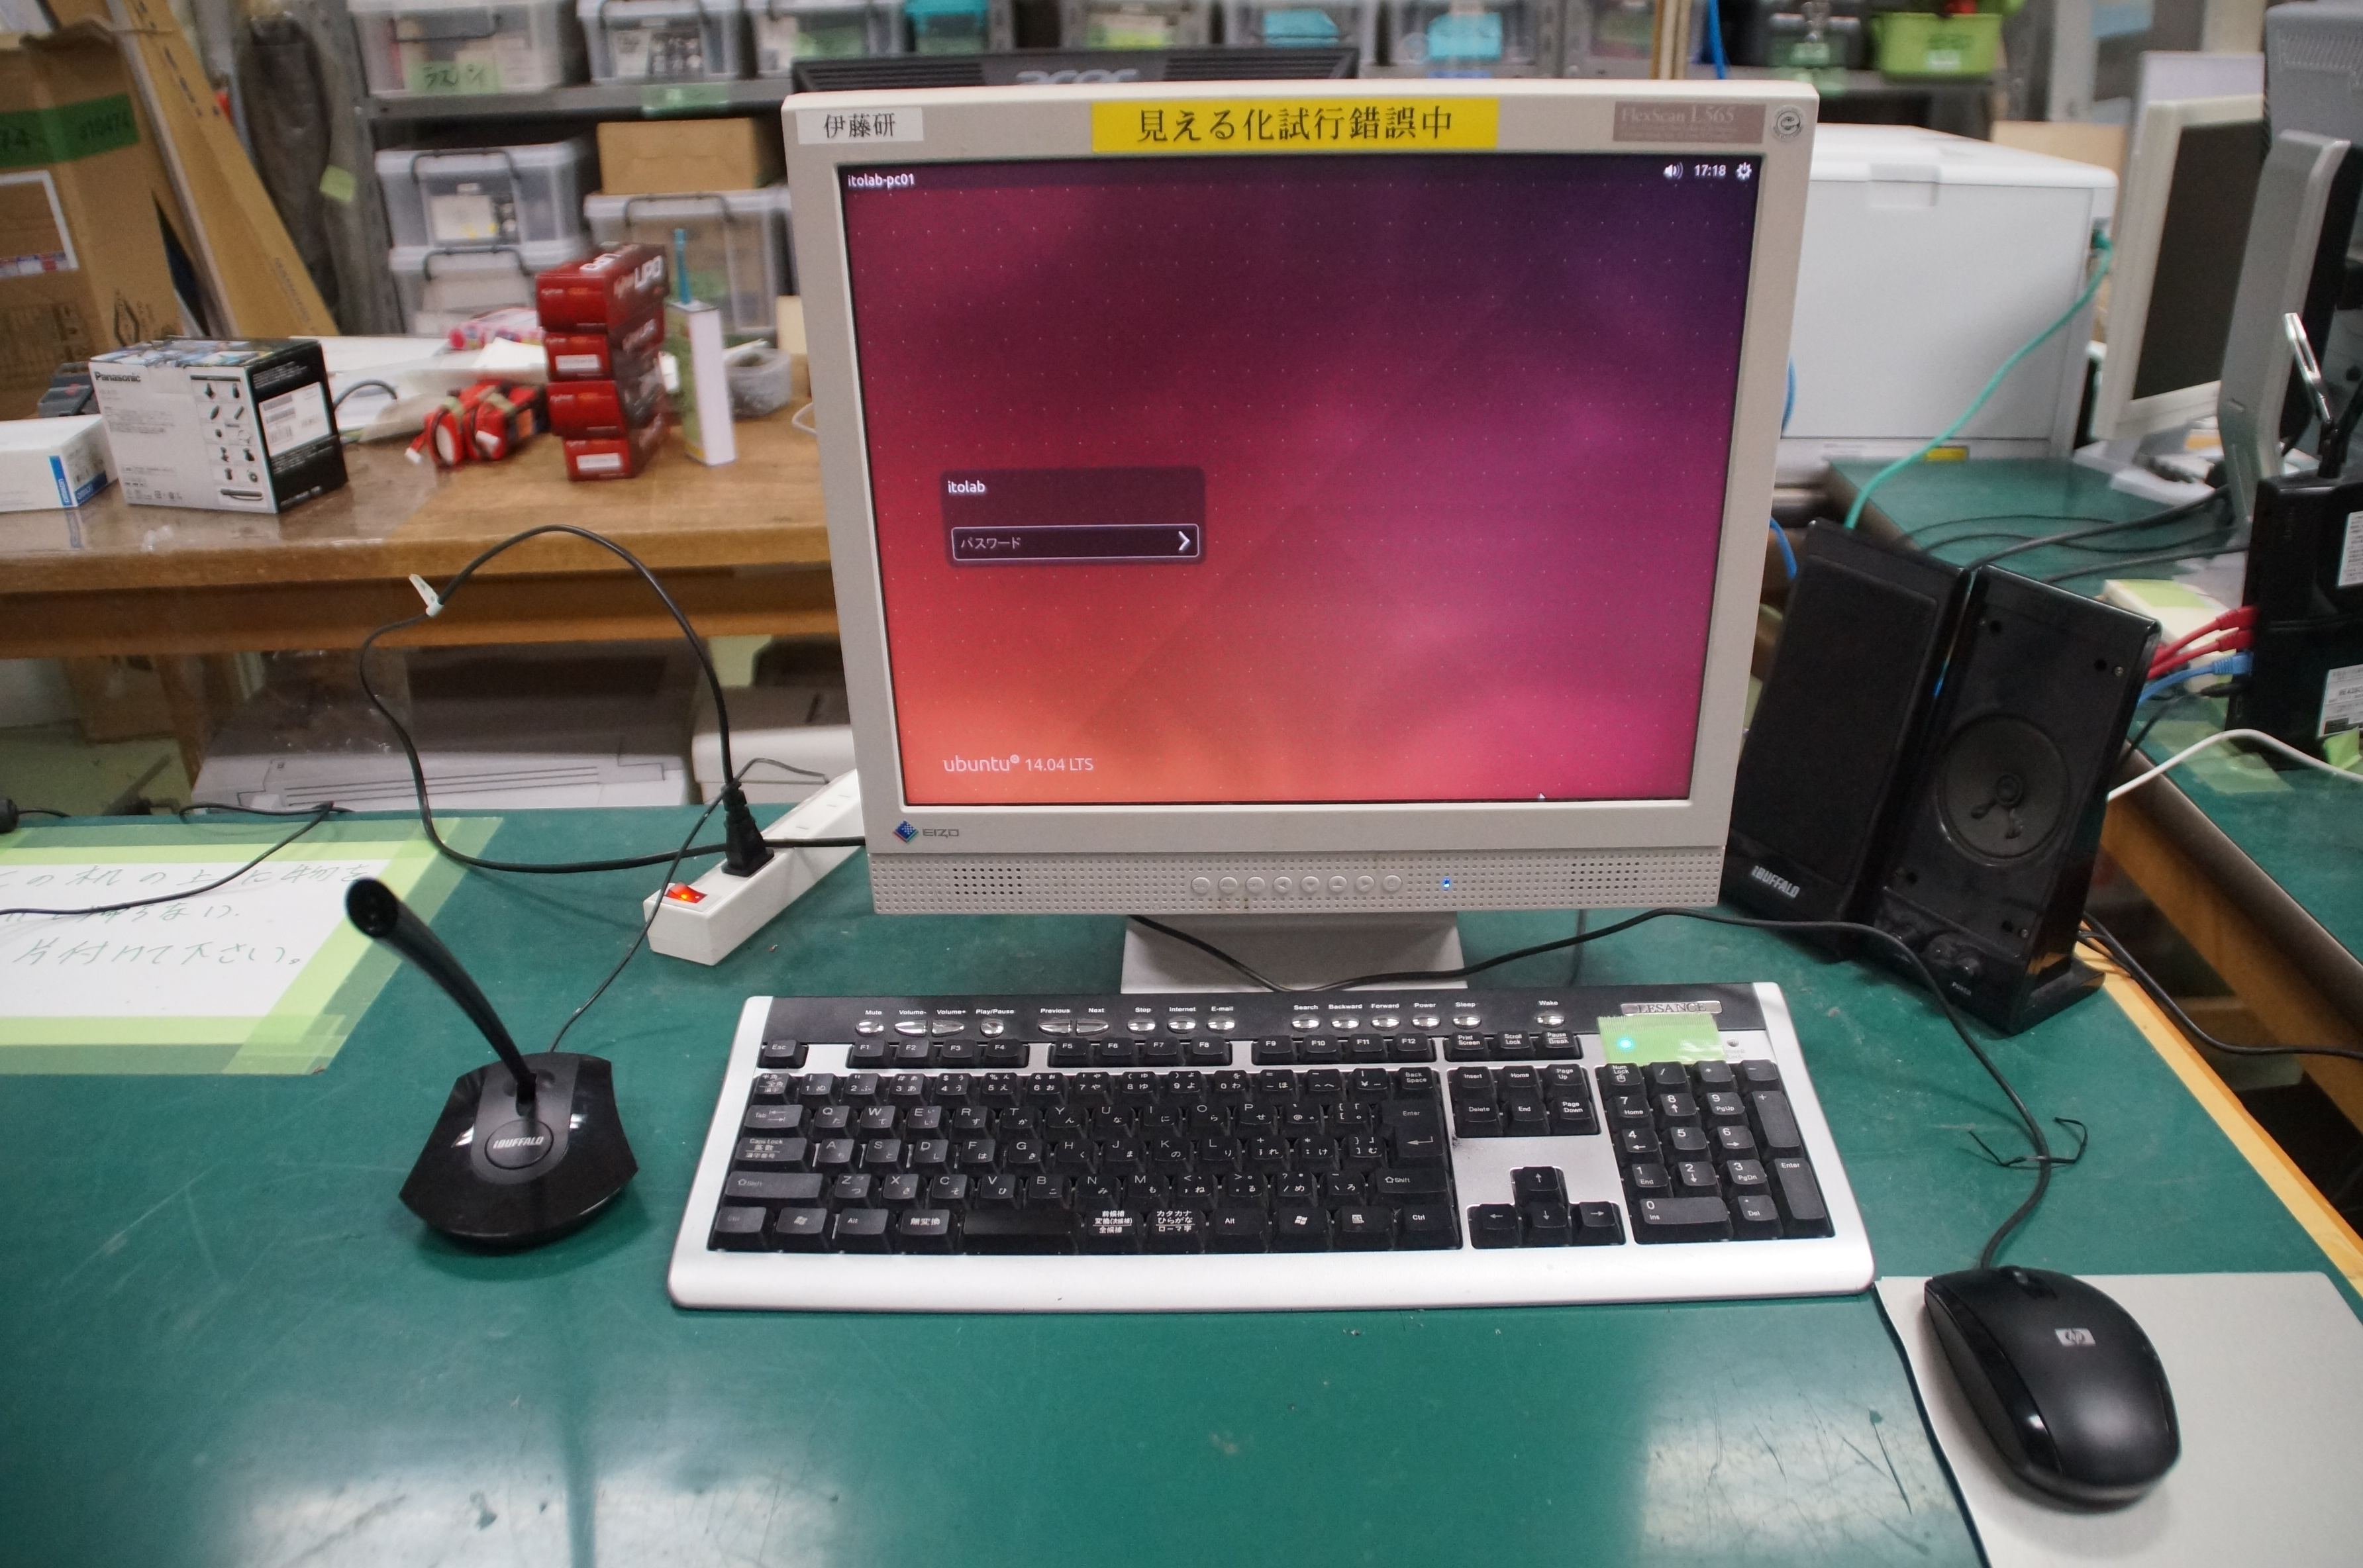
\includegraphics[width=35mm]{img/robo.JPG}
\caption{使用したシステム}
\label{fig:robot}
\end{center}
\end{figure}


\subsection{Julius}
Juliusは,音声認識システムの開発・研究のためのオープンソースの高性能な汎用大語彙連続音声認識エンジンである.数万語彙の連続音声認識を一般のPC上でほぼ実時間で実行できる.また,高い汎用性を持ち,発音辞書や言語モデル・音響モデルなどの音声認識の各モジュールを組み替えることで,様々な幅広い用途に応用できる.[1]Juliusはコマンド1つで起動させることができ,オプションでサーバモードで使用できるため,今回はサーバモードで起動しクライアント側で認識した単語に対応した音声を発生させることを目指す.


\subsection{Open-JTalk}
Open-JTalkは,日本語テキストを音声に変換するシステムである.ここではC言語のなかでsystem関数を使用し,音声を発するためにWAVファイルとして音声を保存するために使用する.


\section{音声認識実験}
\subsection{実験の目的}
音声認識実験ではJuliusを使用して音声を認識させ,認識した回数の平均をとる事を目的とする.


\subsection{実験の手順}

\begin{enumerate}
 \item マイクを実装したパソコンを使用し,Juliusを端末より起動させる.
 \item Juliusを使用し,禁煙です,吸わないです,吸いません,喫煙です,吸います5つの単語の認識を行う.
 \item 100回分の認識結果を集計する.
\end{enumerate}

\subsection{実験の結果}
Juliusを用いて音声を入力し,認識することを確認した.また音声認識実験で得られた認識率を計算した結果,禁煙が99%,喫煙が100%,吸いますが100%,吸いませんが30%,吸わないですが100%という結果が得られた.認識率を算出した際に得られたグラフを図\ref{fig:result}に示す.


\begin{figure}[htbp]
\begin{center}
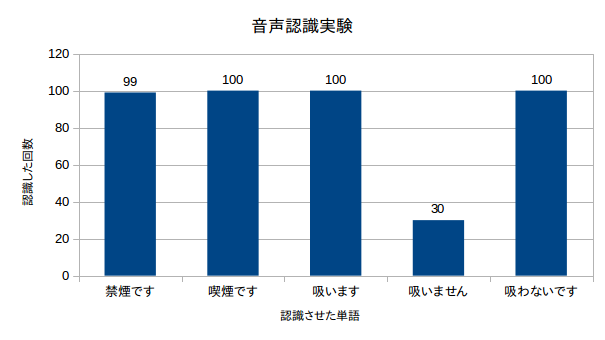
\includegraphics[width=35mm]{img/result.png}
\caption{認識結果グラフ}
\label{fig:result}
\end{center}
\end{figure}


\subsection{考察}
前述の音声認識実験での結果より認識率が99%,30%の単語が存在するという点から雑音が混入した結果ではないかと考えられる.また100人のうち,70人の方が誤認識をする可能性も考えられるため,ノイズカットも必要になるのではないかと考えられる.


\section{おわりに}
本研究ではロボットに音声認識をさせることで人件費の削減につなげられるのではないかと考え,JuliusやOpen-JTalkで音声の入出力を行うことと決めJuliusでの音声の認識やOpen-JTalkで作成した音声の出力に成功した.今後は認識率を高めるためより多くの被研究者を実験対象とし,認識率の算出やノイズカットを施したJuliusを使用して音声認識実験を行う.その後音声を認識したあとにTCP/IPを経由させて認識した単語に対応した音声を発生させる.また,音声合成を使用して作成した音声をお客様が聴きやすい音声となるように音のピッチや高さなどの改良も行う.


\begin{thebibliography}{1}
\bibitem{キー1} 第7章 言語モデル・https://julius.osdn.jp/juliusbook/ja/desc\_lm.html・2016/09/02閲覧
%%%%%%%%%%%%%%%%%%%%%%%%%%%%%%%%%%%%%%%%%%%%%%%%%%%%%%%%%%%%%%%%%%%%%%%%%%%%%%%%%


\end{document}
